\section{Schichtenmodelle}

\begin{defi}{Netzwerkprotokoll}
    Ein \emph{Netzwerkprotokoll}  ist ein Kommunikationsprotokoll für den Austausch von Daten zwischen Computern bzw. Prozessen, die in einem Rechnernetz miteinander verbunden sind (verteiltes System).

    Der Austausch von Nachrichten erfordert häufig ein Zusammenspiel verschiedener Protokolle, die unterschiedliche Aufgaben übernehmen.

    Um die damit verbundene Komplexität beherrschen zu können, werden die einzelnen Protokolle in Schichten organisiert.
    Im Rahmen einer solchen Architektur gehört jedes Protokoll einer bestimmten Schicht an und ist für die Erledigung der speziellen Aufgaben zuständig\footnote{beispielsweise Übermitteln an einen bestimmten Knoten – Schicht 2}.

    Protokolle höherer Schichten verwenden Dienste von Protokollen tieferer Schichten.\footnote{Schicht 3 bildet ein logisches Netzwerk und verwendet Schicht 2 für die physische Zustellung.}
    Zusammen bilden die so strukturierten Protokolle einen Protokollstapel.
\end{defi}

\subsection{ISO/OSI-Referenzmodell}

\begin{defi}{ISO/OSI-Referenzmodell}
    Das \emph{ISO/OSI-Referenzmodell} ist ein Referenzmodell für Netzwerkprotokolle als Schichtenarchitektur.

    Zweck des OSI-Modells ist es, Kommunikation über unterschiedlichste technische Systeme hinweg zu beschreiben und die Weiterentwicklung zu begünstigen.
    Dazu definiert dieses Modell sieben aufeinanderfolgende Schichten (layers) mit jeweils eng begrenzten Aufgaben. In der gleichen Schicht mit klaren Schnittstellen definierte Netzwerkprotokolle sind einfach untereinander austauschbar, selbst wenn sie wie das Internet Protocol eine zentrale Funktion haben.

    \centering
    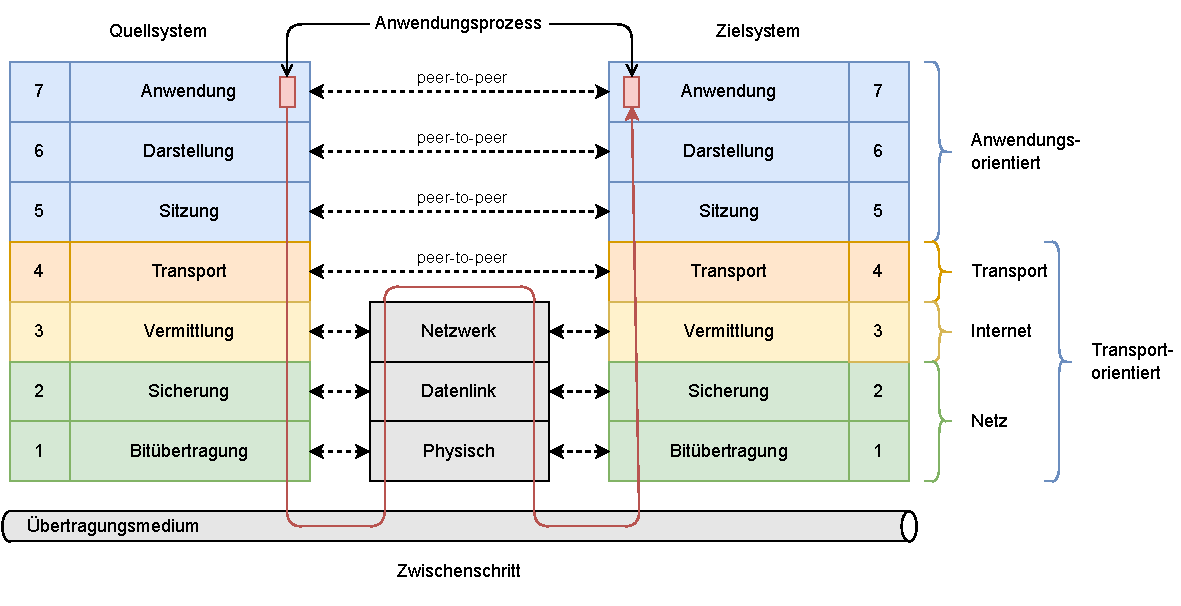
\includegraphics[width=\textwidth]{includes/figures/defi_iso_osi.pdf}
\end{defi}

\begin{defi}{Interaktion zwischen Schichten}
    Eine Schicht $(n-1)$ bietet der über ihr liegenden Schicht $n$ Dienste an.

    Dabei versieht Schicht $n$ ihre Nachricht mit Kontrollinformationen (Header) und versendet alles zusammen als \emph{Protocal Data Unit (PDU)}.

    Zwei Kommunikationspartner auf Schicht $n$ tauschen PDUs aus und nutzen dazu die Dienste der nächsttieferen Schicht $(n-1)$.

    Für Schicht $(n-1)$ sind diese PDUs die zu übertragenen Daten.

    \centering
    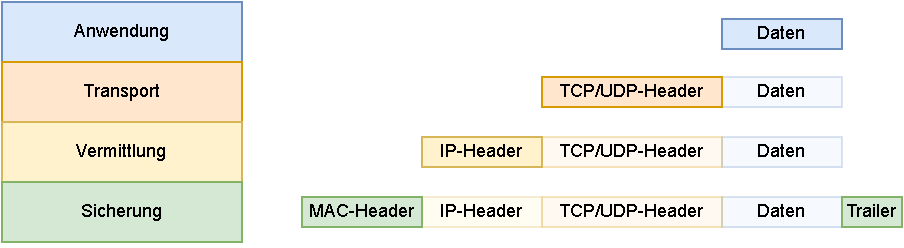
\includegraphics[width=\textwidth]{includes/figures/defi_header_kapselung.pdf}
\end{defi}

\begin{defi}{Schicht 7 - Anwendungsschicht (Application Layer)}
    Dienste, Anwendungen und Netzmanagement.

    Die \emph{Anwendungsschicht} stellt Funktionen für die Anwendungen zur Verfügung.

    Diese Schicht stellt die Verbindung zu den unteren Schichten her.

    Auf dieser Ebene findet auch die Datenein- und ausgabe statt.
    Die Anwendungen selbst gehören nicht zur Schicht.
\end{defi}

\begin{defi}{Schicht 6 - Darstellungsschicht (Presentation Layer)}
    Die \emph{Darstellungsschicht} setzt die systemabhängige Darstellung der Daten (z. B. ASCII, Unicode) in eine unabhängige Form um und ermöglicht somit den syntaktisch korrekten Datenaustausch zwischen unterschiedlichen Systemen.

    Auch Aufgaben wie die Datenkompression und die Verschlüsselung gehören zur Schicht 6.

    Die Darstellungsschicht gewährleistet, dass Daten, die von der Anwendungsschicht eines Systems gesendet werden, von der Anwendungsschicht eines anderen Systems gelesen werden können.

    Falls erforderlich, agiert die Darstellungsschicht als Übersetzer zwischen verschiedenen Datenformaten, indem sie ein für beide Systeme verständliches Datenformat, die ASN.1 (Abstract Syntax Notation One), verwendet.
\end{defi}

\begin{defi}{Schicht 5 - Sitzungsschicht (Session Layer)}
    Die \emph{Sitzungsschicht} sorgt für die Prozesskommunikation zwischen zwei Systemen.

    Um Zusammenbrüche der Sitzung und ähnliche Probleme zu beheben, stellt die Sitzungsschicht Dienste für einen organisierten und synchronisierten Datenaustausch zur Verfügung.
    Zu diesem Zweck werden Wiederaufsetzpunkte, so genannte Fixpunkte (Check Points) eingeführt, an denen die Sitzung nach einem Ausfall einer Transportverbindung wieder synchronisiert werden kann, ohne dass die Übertragung wieder von vorne beginnen muss.
\end{defi}

\begin{defi}{Schicht 4 - Transportschicht (Transport Layer)}
    Zu den Aufgaben der \emph{Transportschicht} zählt die Segmentierung des Datenstroms, die Stauvermeidung (congestion avoidance) und die Sicherstellung einer fehlerfreien Übertragung.

    Die Transportschicht bietet den anwendungsorientierten Schichten 5 bis 7 einen einheitlichen Zugriff, so dass diese die Eigenschaften des Kommunikationsnetzes nicht zu berücksichtigen brauchen.
\end{defi}

\begin{defi}{Schicht 3 - Vermittlungsschicht (Network Layer)}
    Die \emph{Vermittlungsschicht} sorgt bei leitungsorientierten Diensten für das Schalten von Verbindungen und bei paketorientierten Diensten für die Weitervermittlung von Datenpaketen sowie die Stauvermeidung (congestion avoidance).

    Die Datenübertragung geht in beiden Fällen jeweils über das gesamte Kommunikationsnetz hinweg und schließt die Wegsuche (Routing) zwischen den Netzwerkknoten ein.

    Da nicht immer eine direkte Kommunikation zwischen Absender und Ziel möglich ist, müssen Pakete von Knoten, die auf dem Weg liegen, weitergeleitet werden.
    Weitervermittelte Pakete gelangen nicht in die höheren Schichten, sondern werden mit einem neuen Zwischenziel versehen und an den nächsten Knoten gesendet.

    Zu den wichtigsten Aufgaben der Vermittlungsschicht zählt das Bereitstellen netzwerkübergreifender Adressen, das Routing bzw. der Aufbau und die Aktualisierung von Routingtabellen und die Fragmentierung von Datenpaketen.

    Das Internet Protocol gehört zu dieser Schicht.
\end{defi}

\begin{defi}{Schicht 2 - Sicherungsschicht (Data Link Layer)}
    Aufgabe der \emph{Sicherungsschicht} ist es, eine zuverlässige, das heißt weitgehend fehlerfreie Übertragung zu gewährleisten und den Zugriff auf das Übertragungsmedium zu regeln. Dazu dient das Aufteilen des Bitdatenstromes in Blöcke (Frames) und das Hinzufügen von Prüfsummen im Rahmen der Kanalkodierung.
    So können fehlerhafte Blöcke vom Empfänger erkannt und entweder verworfen oder sogar korrigiert werden.

    Eine Datenflusskontrolle ermöglicht es, dass ein Empfänger dynamisch steuert, mit welcher Geschwindigkeit die Gegenseite Blöcke senden darf.

    Das Ethernet-Protokoll beschreibt sowohl Schicht 1 als auch Schicht 2, wobei auf dieser als Zugriffskontrolle CSMA/CD zum Einsatz kommt.
\end{defi}

\begin{defi}{Schicht 1 - Bitübertragungsschicht (Physical Layer)}
    Die \emph{Bitübertragungsschicht} ist die unterste Schicht.

    Diese Schicht stellt mechanische, elektrische, physikalische und weitere funktionale Hilfsmittel zur Verfügung, um physische Verbindungen zu aktivieren bzw. zu deaktivieren, sie aufrechtzuerhalten und Bits darüber zu übertragen. Das können zum Beispiel elektrische Signale, optische Signale (Lichtleiter, Laser), elektromagnetische Wellen (drahtlose Netze) oder Schall sein.

    Die gemeinsame Nutzung eines Übertragungsmediums kann auf dieser Schicht durch statisches Multiplexen oder dynamisches Multiplexen erfolgen. Dies erfordert neben den Spezifikationen bestimmter Übertragungsmedien (zum Beispiel Kupferkabel, Lichtwellenleiter, Stromnetz) und der Definition von Steckverbindungen noch weitere Elemente.
\end{defi}

\subsection{TCP/IP-Referenzmodell}

\begin{defi}{TCP/IP-Referenzmodell}
    Das \emph{TCP/IP-Referenzmodell} ist eine protokollunabhängige Ausmodellierung des konzeptionellen ISO/OSI-Modells.

    \begin{center}
        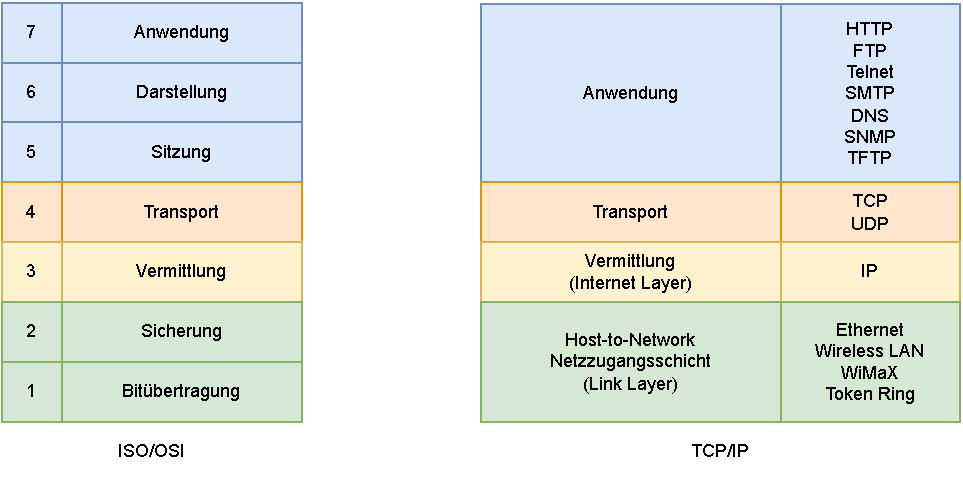
\includegraphics[width=0.75\textwidth]{includes/figures/defi_tcp_ip.pdf}
    \end{center}

    Die einzelnen Schichten erfüllen folgende Funktionen:
    \begin{itemize}
        \item Die \emph{Netzzugangsschicht} ist im TCP/IP-Referenzmodell spezifiziert, enthält jedoch keine Protokolle der TCP/IP-Familie.
              Sie ist vielmehr als Platzhalter für verschiedene Techniken zur Datenübertragung von Punkt zu Punkt zu verstehen.
        \item Die \emph{Internetschicht} ist für die Weitervermittlung von Paketen und die Wegwahl (Routing) zuständig.
              Auf dieser Schicht und der darunterliegenden Schicht werden Direktverbindungen betrachtet.
              Die Aufgabe dieser Schicht ist es, zu einem empfangenen Paket das nächste Zwischenziel zu ermitteln und das Paket dorthin weiterzuleiten.
              Kern dieser Schicht ist das Internet Protocol (IP) in der Version 4 oder 6.
        \item Die \emph{Transportschicht} ermöglicht eine Ende-zu-Ende-Kommunikation. Das wichtigste Protokoll dieser Schicht ist das Transmission Control Protocol (TCP), das Verbindungen zwischen jeweils zwei Netzwerkteilnehmern zum zuverlässigen Versenden von Datenströmen herstellt.
        \item Die \emph{Anwendungsschicht} umfasst alle Protokolle, die mit Anwendungsprogrammen zusammenarbeiten und die Netzwerkinfrastruktur für den Austausch anwendungsspezifischer Daten nutzen.
    \end{itemize}
\end{defi}